\section{Introduction}

Today, changing what a neural network does almost always means training it. You collect examples, run gradient descent, and get back a change spread across millions of parameters that nobody can read. A recent line of work offers a different route. A capable language model, the \emph{programmer}, reads another network's weights, runs a handful of forward passes, works out how the computation goes, and writes the change directly into the weights~\citep{takehi2026sparks}. In the original demonstration, the programmer removed one direction from 131,072 weights in two MLP layers of Qwen3.5-0.8B. That stopped the model looping on maths problems and raised MATH-500 accuracy from 7.9\% to 48.1\%. No gradients were involved, and the fix could be read and checked. Follow-up work has applied the idea to larger language models, biosignal classifiers and game-playing networks~\citep{hu2026exploring,varam2026mixed,lehmann2026compiling}.

If this \emph{weight-space programming} (WSP) worked broadly, it would change how models are patched. Edits could be small enough to review, cheap in GPU time, and built from a few thousand labelled examples rather than a training run. But most evidence so far reports what programming achieved, not how it compares with the obvious alternative; the one direct comparison covers a single published patch on one task family~\citep{yang2026writing}. Someone holding a pretrained model that misbehaves needs to decide whether to program it or fine-tune it. That decision turns on two questions:
\begin{enumerate}
  \item \textbf{When does programming work, compared with fine-tuning?} The repair above rearranged knowledge the model already had. Can a programmer also add knowledge the model lacks? And where it can, how does it compare with gradient training on the same task and the same model?
  \item \textbf{What does an edit cost?} An edit that fixes the target task might break everything else, and measuring only the target task would never show it.
\end{enumerate}

\paragraph{How we test it.} We built a comparison in which one factor varies: how much of the needed knowledge the base model already has. Four five-option tasks span the range:
\begin{itemize}
  \item \textbf{SST-5 sentiment}~\citep{socher2013sst}. The model knows this and reads it out correctly, though imperfectly.
  \item \textbf{SST-5 inverted.} The same prompts with mirrored labels. The model knows the sentiment but reads it out backwards.
  \item \textbf{Twin-2K}~\citep{toubia2025twin}. Predicting a real person's survey answer. The model knows what people in general tend to say, but little about individuals.
  \item \textbf{Fictional facts.} Questions about 300 invented people, with no context. The model cannot know these.
\end{itemize}
A linear probe on the base model's activations measures how much of each answer is already there. Everything else is held fixed: the model, the answer format, the budget of 50 forward passes, and a written brief that every programmer receives. Each programmer is an independent Claude agent, and an independent auditor checks every run afterwards. The baseline is LoRA~\citep{hu2022lora}. The main model is Qwen2.5-1.5B-Instruct~\citep{qwen2025}. We repeat the key experiments on SmolLM2-1.7B-Instruct, a different model family.

\paragraph{What we expected, and what happened.} We expected programming to work in proportion to what the model already knows: good at redirecting, unable to add. The first half held.
\begin{itemize}
  \item \textbf{Mirrored labels: every programmer found the same fix.} All five programmers who attempted the task, across two programmer models and both base models, swapped the embeddings of `` negative'' and `` positive''. A control swap of two unrelated words did nothing.
  \item \textbf{The swap matched LoRA, and was more reliable than its default configuration.} Default LoRA failed to learn the task on two of three seeds.
\end{itemize}
The second half did not hold.
\begin{itemize}
  \item \textbf{Programmers added knowledge by compiling it.} Faced with facts the model could not know, they turned the training labels into explicit lookup circuits that recalled every fact under unseen wordings. On survey answers, a similar circuit beat LoRA.
  \item \textbf{Those circuits break the model.} After them, the model scores at chance on MMLU and almost never predicts the next token of ordinary text (0--0.1\% top-1, against 46\%). This held on both model families (Figure~\ref{fig:tradeoff}).
  \item \textbf{Through edits mostly keep the model intact.} An edit that stored the facts through the model's own memory pathway recalled fewer of them (77\%), but left the model as capable as before, just as LoRA does.
\end{itemize}

\begin{figure}[t]
\centering
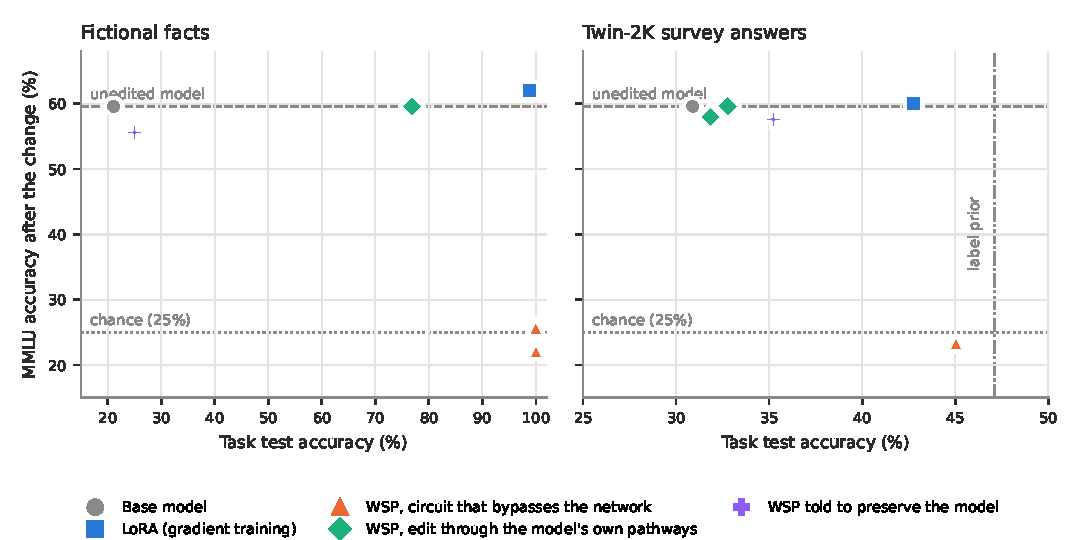
\includegraphics[width=\linewidth]{figures/tradeoff.pdf}
\caption{The trade-off behind the best weight-space programming results (Qwen2.5-1.5B). Each point is one way of teaching the model a task it cannot already do. Horizontal axis: test accuracy on that task. Vertical axis: the model's MMLU accuracy afterwards. Circuits that bypass the network (orange) reach the highest task accuracy and leave the model at chance on MMLU. Edits through the model's own pathways (green), edits from a programmer told to preserve the model (purple) and LoRA (blue) keep MMLU near the unedited level.}
\label{fig:tradeoff}
\end{figure}

\paragraph{Two follow-up experiments changed the picture.}
\begin{itemize}
  \item \textbf{Telling the programmer to preserve the model changes the edit it builds.} The brief said nothing about side effects, so we added a requirement to preserve the model's other abilities. On survey answers, the same programmer then switched from a destructive circuit to a gated edit that gains 4.3 points and leaves the model's other abilities unchanged. On facts, it could not find an edit that both added knowledge and passed the preserve check.
  \item \textbf{Programming and fine-tuning combine.} Running LoRA on top of a programmed edit raised facts accuracy to 99.0--99.7\% with 4,000 training examples. LoRA alone needed about ten times as much data. On mirrored labels the combination reached 57--59\%, well above either method alone.
\end{itemize}

\paragraph{So what.} For anyone deciding how to change a model, the results give a usable map:
\begin{itemize}
  \item \textbf{Redirect.} When the model has the knowledge but uses it wrongly, program it. The fixes are tiny, readable and reproducible, and more reliable than default fine-tuning.
  \item \textbf{Compile.} When the answer is a table that can be written from the labels, programming matches or beats fine-tuning. But its most accurate route disables the model, so the edit must be checked, and the brief must ask for preservation.
  \item \textbf{Learn.} When the improvement needs a better mapping from inputs to answers, fine-tune.
  \item \textbf{Combine.} In both regimes where we tried it, a programmed edit was a good starting point for fine-tuning, and the combined models kept general ability.
\end{itemize}
For anyone evaluating edits, target-task accuracy is not enough. The highest-scoring edits are the most damaging. Raw perplexity misleads in the opposite direction: it flags harmless temperature changes as damage. We propose a small side-effect protocol that avoids both traps.

\paragraph{Contributions.}
\begin{enumerate}
  \item A controlled comparison of weight-space programming with gradient fine-tuning on pretrained language models that varies how much the model already knows, with 20 independent programmer runs across two programmer models and two model families. Every edit and log is released, and every run that produced an edit, apart from an early pilot, is independently audited.
  \item A map of three regimes (redirect, compile, learn), with independent replications. That includes a fix five programmers found separately and three different SST-5 mechanisms that hit the same ceiling.
  \item Evidence that the most accurate programmed edits bypass the network and destroy general ability, on both model families. Edits through the model's pathways do not, and an instruction to preserve the model moves the programmer from one kind to the other.
  \item Evidence that programming and fine-tuning are complementary: a programmed edit fixes both LoRA failure modes we observed, slow storage of new facts and a stuck start on a confidently wrong task. The combined models keep general ability.
  \item An evaluation protocol for weight-space programming: a fixed brief, a ledgered budget, independent audits, and side-effect measures that a temperature change cannot fake.
\end{enumerate}
